\section{Thrust 2: Explainable AI-enabled Software Vulnerability Assessment}
\label{sec:thrust2}

\subsection{Motivating Example}
\label{exe:sec}

%CVE-2021-37714: description
%CVSS Scores

%Input-Output

%Code Change: src/main/java/org/jsoup/parser/HtmlTreeBuilder.java

%Crash-point or infinite loop: HtmlTreeBuilderState.java


Let us present an example from an HTML parser,~named {\em
  jsoup}, and our observations.
%for motivation.
Fig.~\ref{CVSS-tab} displays the information on the vulnerability
CVE-2021-37714 that was reported on {\em jsoup}, and published on
08/18/21.~The change that was deemed to contribute to the
vulnerability were committed at version 1.12.1 to the method
\code{process(Token,HtmlTreeBuilder)} of the
\code{Html\-Tree\-Builder\-State} class (lines 10--11, and 12 of
Fig.~\ref{fig:motiv-code}). That change directly uses the value
returned from \code{reset\-Inser\-tion\-Mode()} as the condition to
insert \code{starTag} (line 13). With this~change, certain input HTML
code with a specific start tag could make the program go to line 16
with a recursive call to the method \code{process(...)}. That~call
resulted in an NullPointerException at line 3 as noted in the
log:~{\em ``java.\-lang.\-Null\-Pointer\-Ex\-ception: Cannot invoke
  "org.\-jsoup.\-nodes.\-Element.\-normalName()" because the return
  value of
  "org.\-jsoup.\-parser.\-HtmlTree\-Builder.\-current\-Element()" is
  null.''}. In other cases, the parser can get stuck, i.e., {\em
  ``loop indefinitely until canceled''} as described in CVE-2021-37714 (Fig.~\ref{CVSS-tab}). Due
to those effects, this vulnerability is considered as {\em a denial of
  service (DoS)}.

\begin{figure}[t]
  \begin{flushleft}
    \footnotesize
\textbf{Vulnerability Details: CVE-2021-37714}\\
\textbf{1. Description}:
{\em jsoup is a Java library for working with HTML. Those using jsoup versions prior to 1.14.2 to parse untrusted HTML or XML may be vulnerable to DOS attacks. If the parser is run on user supplied input, an attacker may supply content that causes the parser to get stuck (loop indefinitely until cancelled), to complete more slowly than usual, or to throw an unexpected exception. This effect may support a denial of service attack. The issue is patched in version 1.14.2. There are a few available workarounds. Users may rate limit input parsing, limit the size of inputs based on system resources, and/or implement thread watchdogs to cap and timeout parse runtimes.
  Publish Date : 2021-08-18 Last Update Date : 2022-02-07}
%\textbf{2. Vulnerability Type(s)}: Denial Of Service
%{\bf 3. CVSS Score:} ...\\
%{\bf 4. Detailed CVSS Grades:}\\
\end{flushleft}
%  \centering
%  \tabcolsep 3pt
%  \scriptsize
%  \begin{tabular}{lll}
%   Vulner. Assess. Type   & Value & Description \\
%      \hline
%    Confidentiality Impact & {\bf None}  & No impact to the confidentiality \\
%    Integrity Impact & {\bf None}  & No impact to the integrity \\
%    Availability Impact & {\bf Partial} & There is reduced performance or\\
%    & & interruptions in availability\\
%    Access Complexity & {\bf Low} & Specialized access conditions or \\
%    & & extenuating circumstances do not exist\\
%    & & Little knowledge is required to exploit\\
%    Authentication & {\bf Not Req} & Authentication is not required \\
%    & & to exploit the vulnerability\\
%    Gained Access & {\bf None}  & No gained access with the vulnerability \\
%    Acccess Vector & {\bf Local} & The vulnerability is in the local parser \\
%    \end{tabular}%
  %  \label{CVSS:tab}%
  \vspace{-16pt}
\caption{Vulnerability Details: CVE-2021-37714}
\label{CVSS-tab}
\end{figure}

%\begin{wrapfigure}{l}{0.5\textwidth}
%	\centering
%	\lstset{
%		numbers=left,
%		numberstyle= \tiny,
%		keywordstyle= \color{blue!70},
%		commentstyle= \color{red!50!green!50!blue!50},
%		frame=shadowbox,
%		rulesepcolor= \color{red!20!green!20!blue!20} ,
%		xleftmargin=1.5em,xrightmargin=0em, aboveskip=1em,
%		framexleftmargin=1.7em,
%                numbersep= 5pt,
%		language=Java,
%    basicstyle=\tiny\ttfamily,
%    numberstyle=\tiny\ttfamily,
%    emphstyle=\bfseries,
%                moredelim=**[is][\color{red}]{@}{@},
%		escapeinside= {(*@}{@*)}
%	}
%	\begin{lstlisting}[]
%// .../jsoup/parser/HtmlTreeBuilderState.java
%boolean process(Token t, HtmlTreeBuilder tb) { ...
%  if (t.isCharacter()&& inSorted( (*@{\color{red}{tb.currentElement().normalName()}@*),InTableFoster)){
%     ...
%     return tb.process(t);
%  }
%  ...
%  } else {
%      tb.popStackToClose(name);
%(*@{\color{orange}{- \quad \quad tb.resetInsertionMode();}@*)
%(*@{\color{orange}{- \quad \quad if (tb.state() == InTable) \{}@*)
%(*@{\color{cyan}{+ \quad \quad if (!tb.resetInsertionMode()) \{}@*)
%         tb.insert(startTag);
%         return true;
%      }
%(*@{\color{red}{\quad \quad \quad return tb.process(t, InHead);}@*)
%      ...
%}
%	\end{lstlisting}
%        \vspace{-15pt}
%        \caption{Code Change at Version 1.12.1 for CVE-2021-37714}
%        \vspace{-6pt}
%        \label{fig:motiv-code}
%\end{wrapfigure}

%     tb.newPendingTableCharacters();
%     tb.markInsertionMode();
%     tb.transition(InTableText);


%vulnerability}.

Fig.~\ref{cvss} shows the Common Vulnerability Scoring System
grades (CVSS) given by security experts for
different \underline{v}ulnerability \underline{a}ssessment
\underline{t}ypes (VATs) for CVE-2021-37714. Due to the above effects,
the availability impact for this~vulnerability is rated as {\em
  Partial} (i.e., for some inputs, there will be reduced performance
and interruptions in available services).

%Recent research~\cite{deepCVA-ase21} has developed a machine learning
%(ML) model that learns from the existing grading from security experts
%to provide the new grading for a committed code change that was deemed
%to be vulnerable. This type of commit-level automated vulnerability
%assessment together with a vulnerability detection (VD) tool are very
%useful in helping developers to early detect and assess the impacts of
%the detected vulnerability as soon as the code is committed.  However,
%the state-of-the-art approach for commit-level vulnerability
%assessment is still limited as explained in the following
%observations.

\begin{figure}
     \centering
     \begin{minipage}{0.45\textwidth}
\centering
\lstset{
		numbers=left,
		numberstyle= \tiny,
		keywordstyle= \color{blue!70},
		commentstyle= \color{red!50!green!50!blue!50},
		frame=shadowbox,
		rulesepcolor= \color{red!20!green!20!blue!20} ,
		xleftmargin=1.5em,xrightmargin=0em, aboveskip=1em,
		framexleftmargin=1.7em,
                numbersep= 5pt,
		language=Java,
    basicstyle=\tiny\ttfamily,
    numberstyle=\tiny\ttfamily,
    emphstyle=\bfseries,
                moredelim=**[is][\color{red}]{@}{@},
		escapeinside= {(*@}{@*)}
	}
	\begin{lstlisting}[]
// .../jsoup/parser/HtmlTreeBuilderState.java
boolean process(Token t, HtmlTreeBuilder tb) { ...
  if (t.isCharacter()&& inSorted( (*@{\color{red}{tb.currentElement().normalName()}@*),InTableFoster)){
     ...
     return tb.process(t);
  }
  ...
  } else {
      tb.popStackToClose(name);
(*@{\color{orange}{- \quad \quad tb.resetInsertionMode();}@*)
(*@{\color{orange}{- \quad \quad if (tb.state() == InTable) \{}@*)
(*@{\color{cyan}{+ \quad \quad if (!tb.resetInsertionMode()) \{}@*)
         tb.insert(startTag);
         return true;
      }
(*@{\color{red}{\quad \quad \quad return tb.process(t, InHead);}@*)
      ...
}
	\end{lstlisting}
         \caption{Code Change v1.12.1 for CVE-2021-37714}
         \label{fig:motiv-code}
     \end{minipage}
     \hfill
     \begin{minipage}{0.5\textwidth}
%          \centering
%\textbf{2. Vulnerability Type(s)}: Denial Of Service

%{\bf 3. CVSS Score:} ...\\

%{\bf 4. Detailed CVSS Grades:}\\
       %  \centering
       \begin{flushleft}
  \tabcolsep 3pt
  \scriptsize
  \begin{tabular}{lll}
   Vulner. Assess. Type   & Value & Description \\
      \hline
    Confidentiality Impact & {\bf None}  & No impact to the confidentiality \\
    Integrity Impact & {\bf None}  & No impact to the integrity \\
    Availability Impact & {\bf Partial} & There is reduced performance or\\
    & & interruptions in availability\\
    Access Complexity & {\bf Low} & Specialized access conditions or \\
    & & extenuating circumstances do not exist\\
    & & Little knowledge is required to exploit\\
    Authentication & {\bf Not Req} & Authentication is not required \\
    & & to exploit the vulnerability\\
    Gained Access & {\bf None}  & No gained access with the vulnerability \\
    Acccess Vector & {\bf Local} & The vulnerability is in the local parser \\
  \end{tabular}%
  \end{flushleft}
    \caption{Detailed CVSS Impact Grades}
         \label{cvss}
     \end{minipage}
\end{figure}

\subsection{Proposed Solution}
\label{overview:sec}



%Figure~\ref{fig:overview} illustrates the overall architecture of
%{\tool}.

\noindent {\tool} has three key components working in three~steps
(Fig.~\ref{fig:overview}).

%\subsubsection*{{\bf Step 1. Multi-version PDG ({\mvpdgxy}) Generation}}

\vspace{2pt}
\subsubsection*{{\bf Step 1. Representing Code Changes and Contexts with Multi-version PDG ({\mvpdgxy})}}
Program Dependence Graph~\cite{pdg} is a directed graph with a
set $N$ of nodes and a set $E$ of edges. A node $n \in N$
represents a program statement or a conditional expression; an edge $e
\in E$ represents the data or control flow among the statements.
A graph representation, called multi-version program
dependence graph ({\mvpdgxy})~\cite{flexeme-fse20} represents the
code changes between two versions $x$ and $y$, before and after the
commit. 

\begin{Definition}[Multi-version Program Dependence Graph] ({\bf {\mvpdgxy}}).
A {\mvpdgxy}~\cite{flexeme-fse20} is a directed graph generated from the
disjoint union of all nodes and edges in the PDGs at versions $x$
and~$y$.
\end{Definition}

%{\mvpdgxy} is a directed graph generated from the disjoint union of
%all nodes and edges in both PDGs at the version $x$ and the version
%$y$ (Figure~\ref{fig:multi-version-pdg}).

%{\mvpdgxy} allows us to capture the program dependencies including data/control
%flows that are crucial in assessing the impacts of a vulnerability.

%Contextualized Embeddings for Code Changes



\vspace{2pt}
\subsubsection*{{\bf Step 2. Graph-based Representation Learning to build Contextualized Embeddings for Code Changes}}

\begin{wrapfigure}{l}{0.5\textwidth}
	\centering
	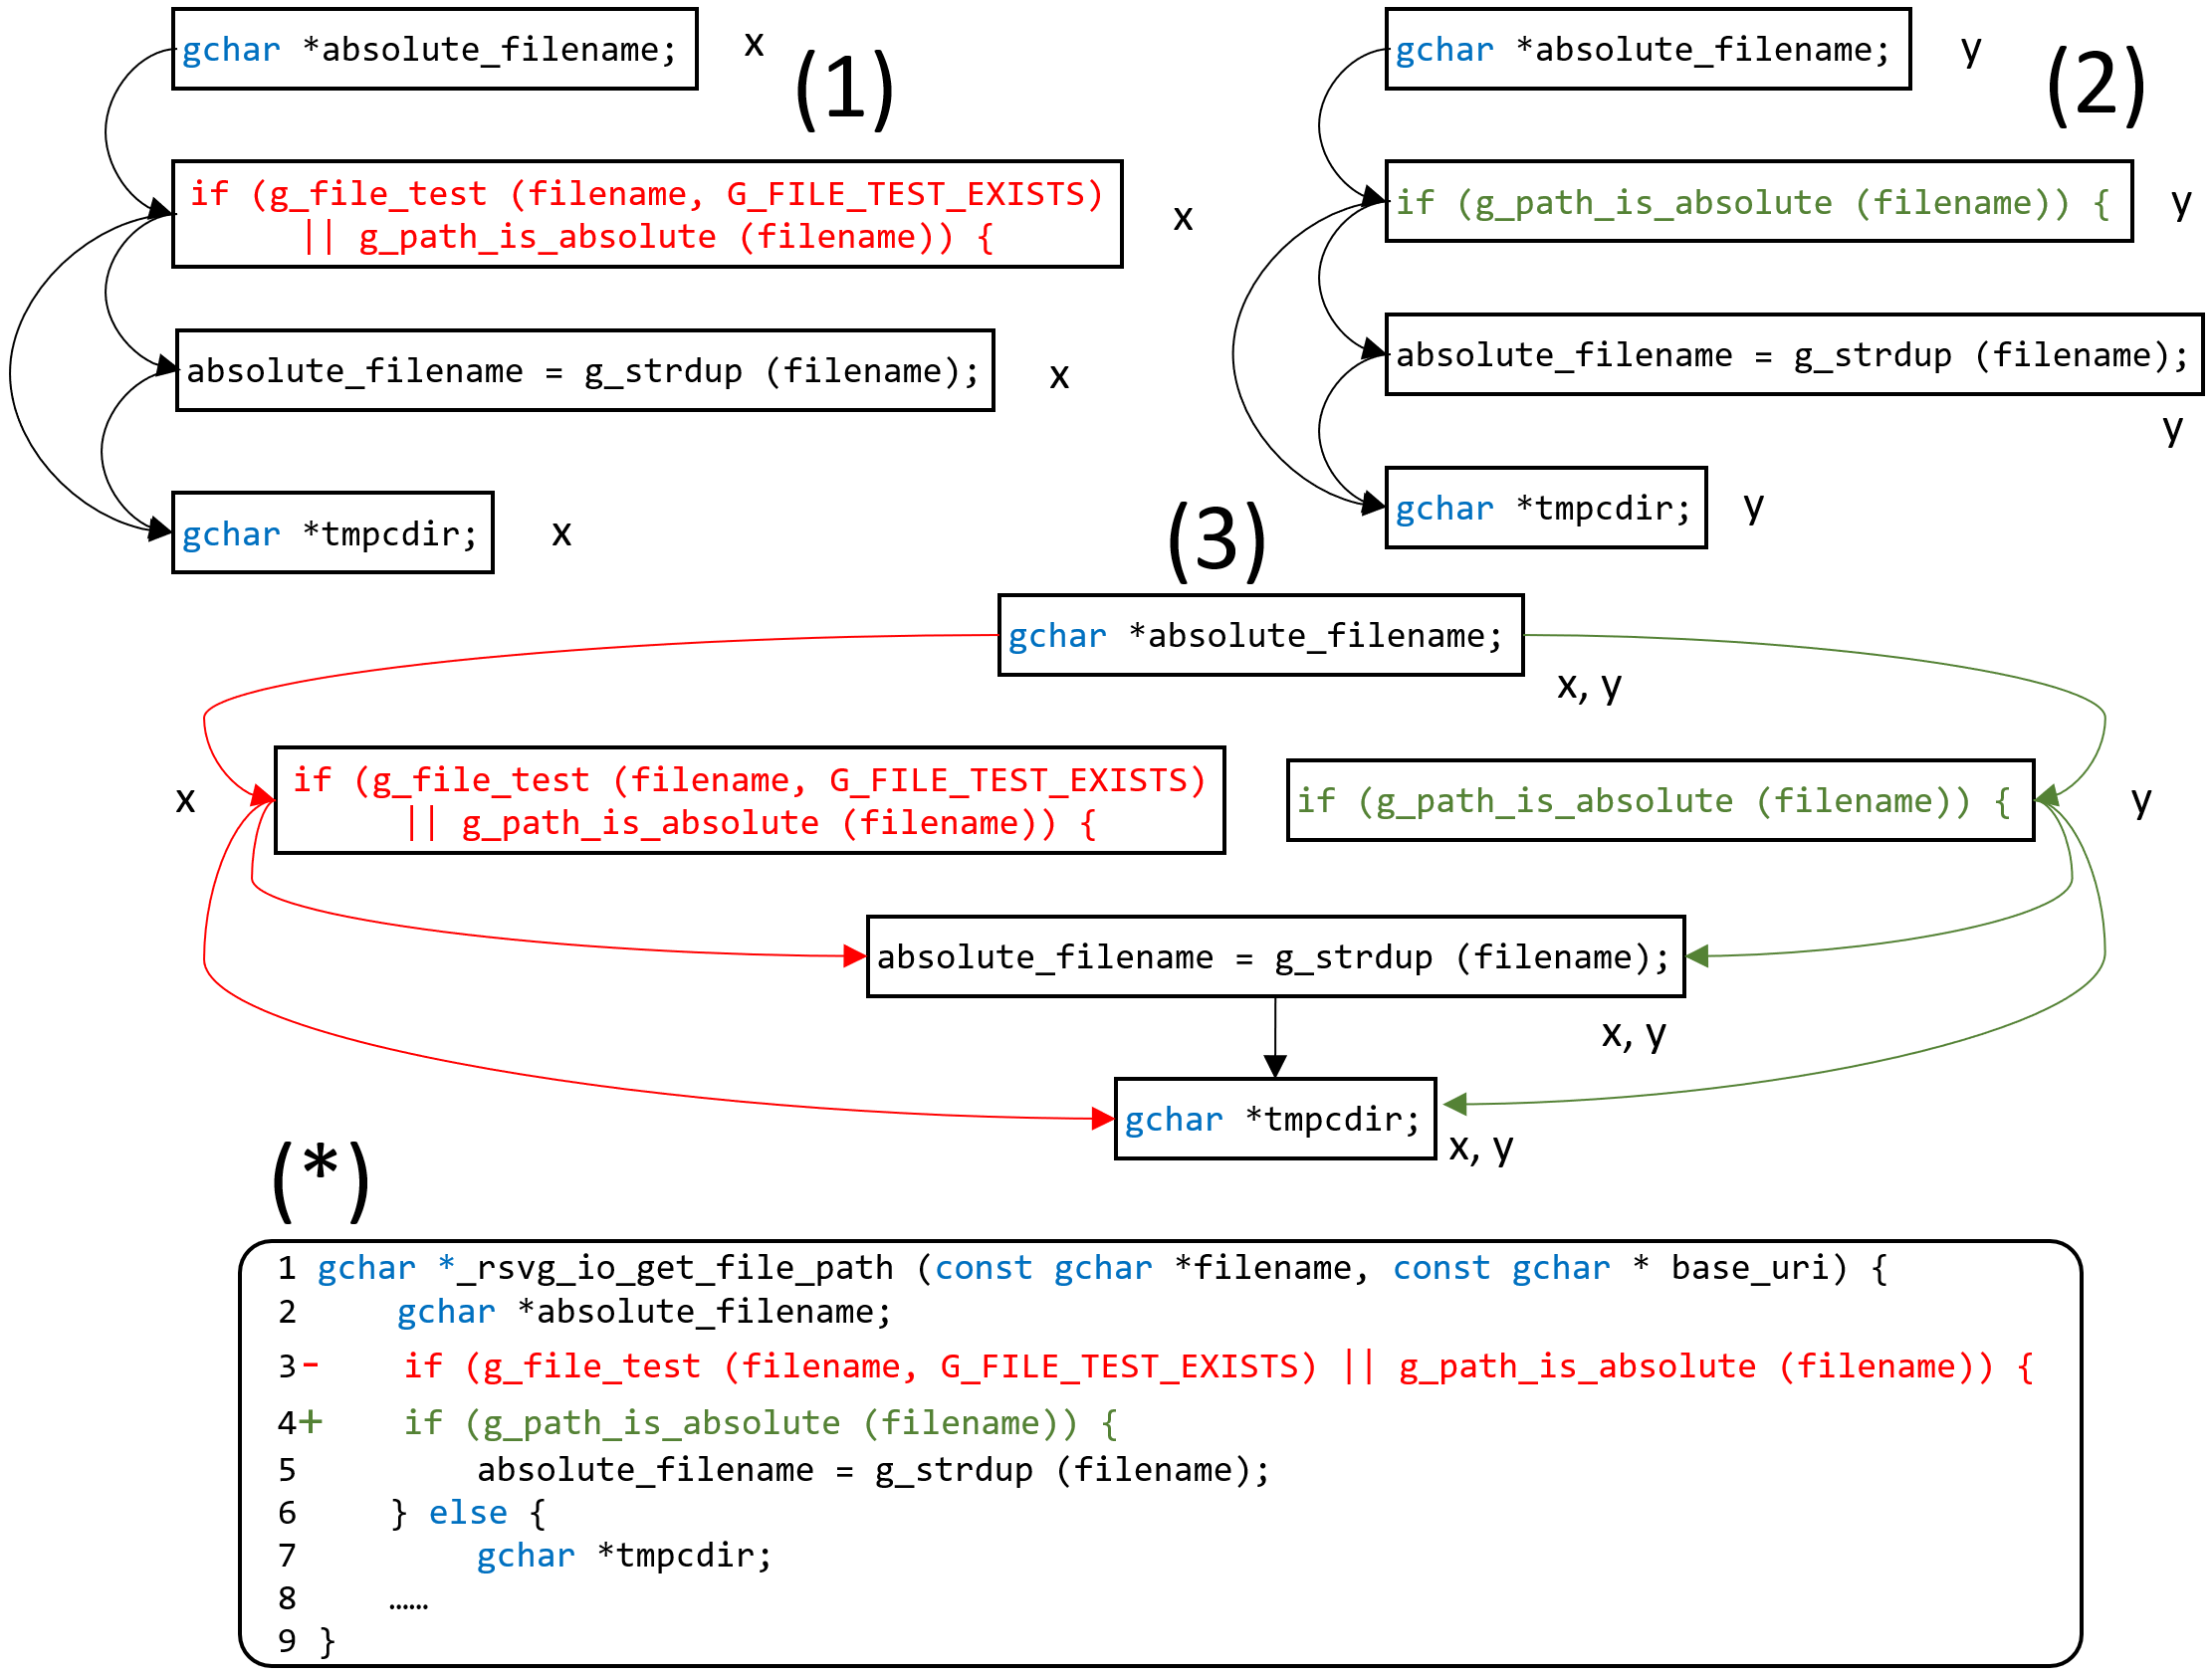
\includegraphics[width=3.4in]{multi-version-pdg.png}
	\caption{Multi-Version Program Dependence Graph}
	\label{fig:multi-version-pdg}
\end{wrapfigure}


We propose a context-aware, graph-based, representation learning model
to learn the contextualized embeddings for the code changes in a
commit that integrate both program dependencies and the contexts. To
build the contextualized embeddings, we leverage the Label,
Graph-based Convolution Network~\cite{label-gcn} to learn the
representation vector $v$ for node $n$ in the graph whose nodes
can have labels. We use labels to denote the nodes at either versions
$x$ or $y$, or at both versions $x$ and $y$.



For a changed node $n_c$, we collect all the un-changed nodes in the
context of $n_c$. The context is defined as the set of all the
un-changed nodes that are $k$-hop neighbors of $n_c$. In the
{\mvpdgxy} in Fig.~\ref{fig:multi-version-pdg}, for the changed
statement at line 4, if $k=1$, the context of that change includes the
statements at lines 2, 5, and 7 (i.e., 1-hop neighbors from line 4).




From the context nodes, we compute the vector representing the context
for a changed node $n_c$ and use it as a weight to represent the
impact of context to build the contextualized embedding for $n_c$.
From those embeddings, we compute the vector for the entire
commit and feed it to
%a SoftMax layer acting as
a classifier to~per\-form assessment classification for each CVSS
assessment type.

%Tien rewrote this para as above
%We collect the vectors of the context nodes into a matrix and use a
%fully connected layer to convert the matrix into a vector $v_{ctx}$ to
%encode the contextual information for the changed node $n_c$. The
%context vector $v_{ctx}$ is used as a weight to represent the impact
%of context on learning to build the contextualized embedding for the
%changed node $n_c$. We next concatenate all the vectors for the all
%the changed nodes $n_c$s into a matrix and use a fully connected layer
%to build the final vector $v^{com}$ for the entire commit. Finally, we
%feed the vector $v^{com}$ to a SoftMax layer acting as a classifier to
%perform assessment classification for each CVSS assessment type.


%\subsubsection{{\bf Step 2. Multi-task Learning-based Vulnerability Assessment Classification}}

%After having the {\mvpdgxy}, this step is mainly used to do the classification for seven different vulnerability assessment types. To achieve that, \tool setups seven separate but similar tasks on seven vulnerability assessment classification problems. Here, we pick one task to explain it in detail.

%The first step of the vulnerability assessment classification is to learn the summarized representation vector for the code changes in the vulnerability bring commit. In this step, \tool uses the Label-GCN \cite{} that can deal with the nodes with multiple labels (suitable for $x$, $y$, and $x,y$ labels in {\mvpdgxy})to learn the representation vector $v$ for each node $n$ in the graph. \tool then picks out all changed nodes in {\mvpdgxy} as a set. For each changed node $n^c$ in this set, \tool firstly collects the representation vector $v^{uc}$ for all unchanged nodes $n^{uc}$ within the $k$-hops in {\mvpdgxy} as the context of the changed node $n^c$. For example, in the {\mvpdgxy} in Figure \ref{fig:multi-version-pdg}, if we regard the statement in $line-4$ is the changed statement that we are focusing on. When $k=1$, the context of it includes the statements in $line-2$, $line-5$, and $line-7$. By concatenating $v^{uc}$ in a new dimension as a matrix, \tool uses a fully connected layer to summarize the matrix into one vector $v^{ctx}$ to represent the context information for the changed node $n^c$. Then, \tool uses the cross product to combine the node representation vector $v^c$ with the context representation vector $v^{ctx}$ to get the final representation vector $v'^c$ for the changed node $n^c$.


%Because the vulnerability assessment we want to get is for the whole vulnerability bring in commits, \tool concatenates $v'^c$ as a matrix and uses a fully connected layer to summarize the final code change representation vector $v^{commit}$. After having the final code change representation vector $v^{commit}$, \tool uses the SoftMax layer as a classifier to do the vulnerability assessment classification based on the $v^{commit}$.

\vspace{2pt}
\subsubsection*{{\bf Step 3. Multi-Task Learning for Assessment Classification}}

\begin{wrapfigure}{l}{0.55\textwidth}
	\centering
	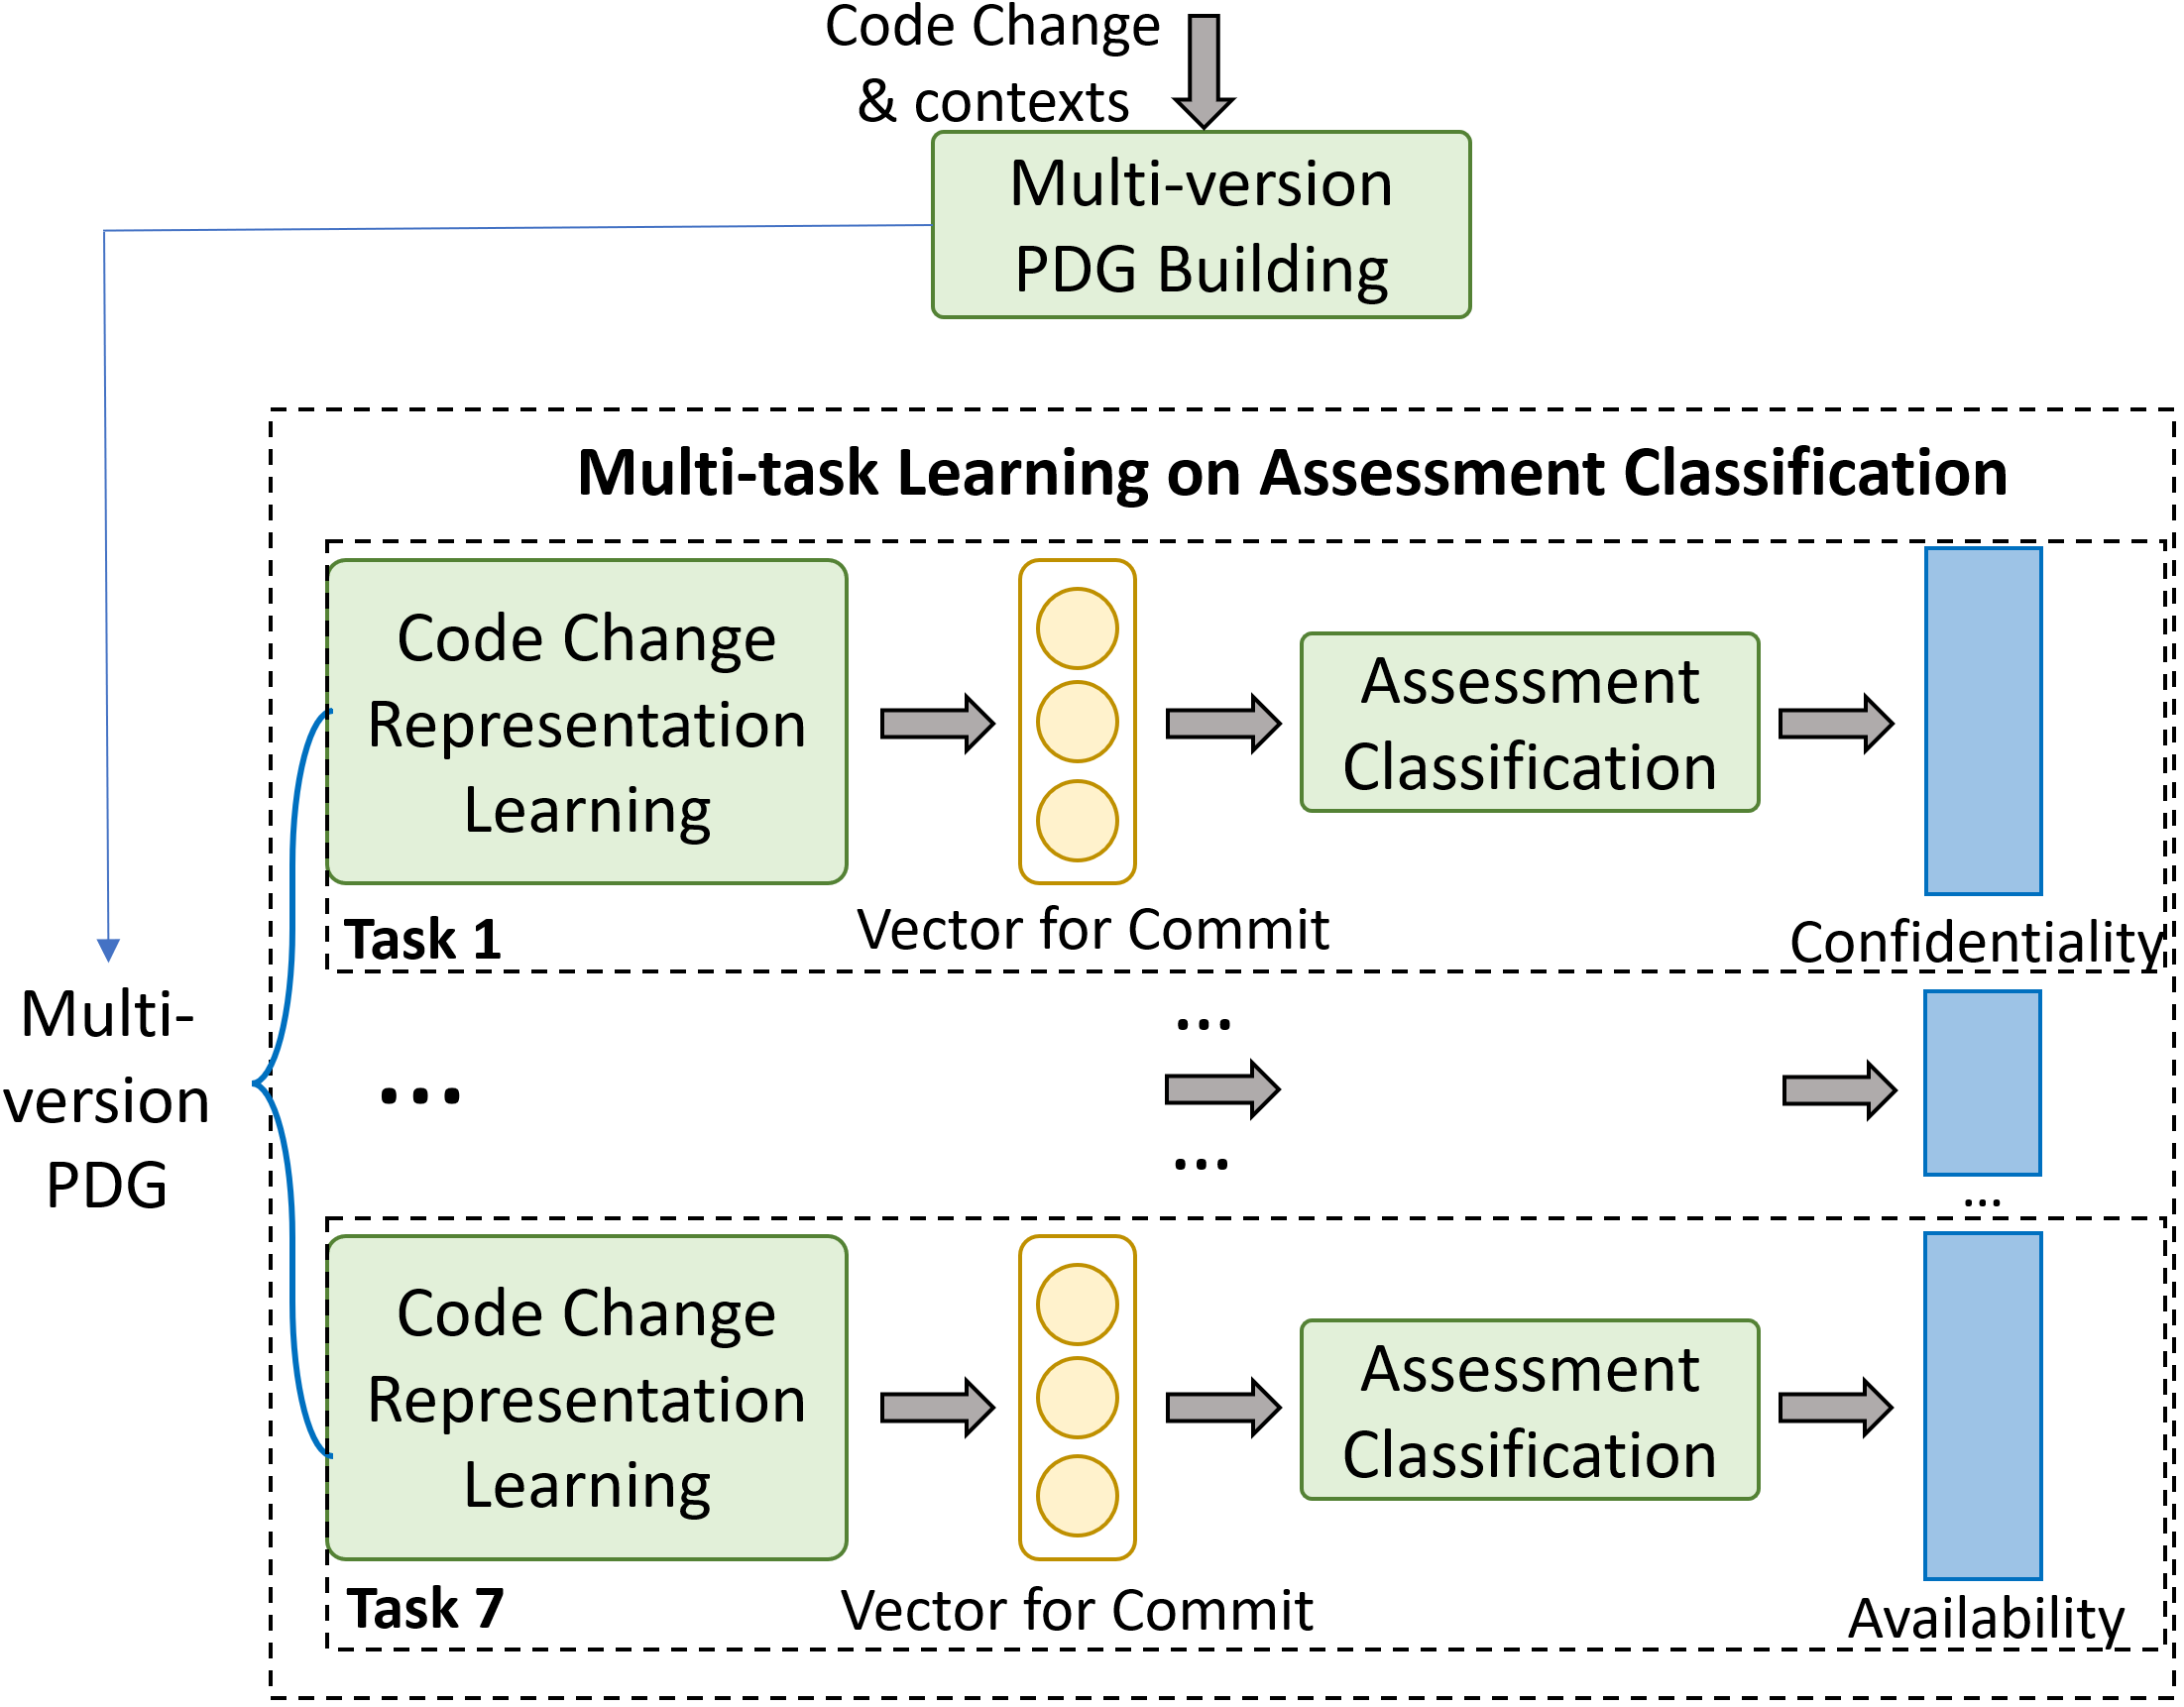
\includegraphics[width=3.4in]{overview-cat.png}
%	\vspace{-6pt}
	\caption{Automated Vulnerability Assessment}
	\label{cat-overview}
\end{wrapfigure}

%\begin{wrapfigure}{l}{0.5\textwidth}
%	\centering
%	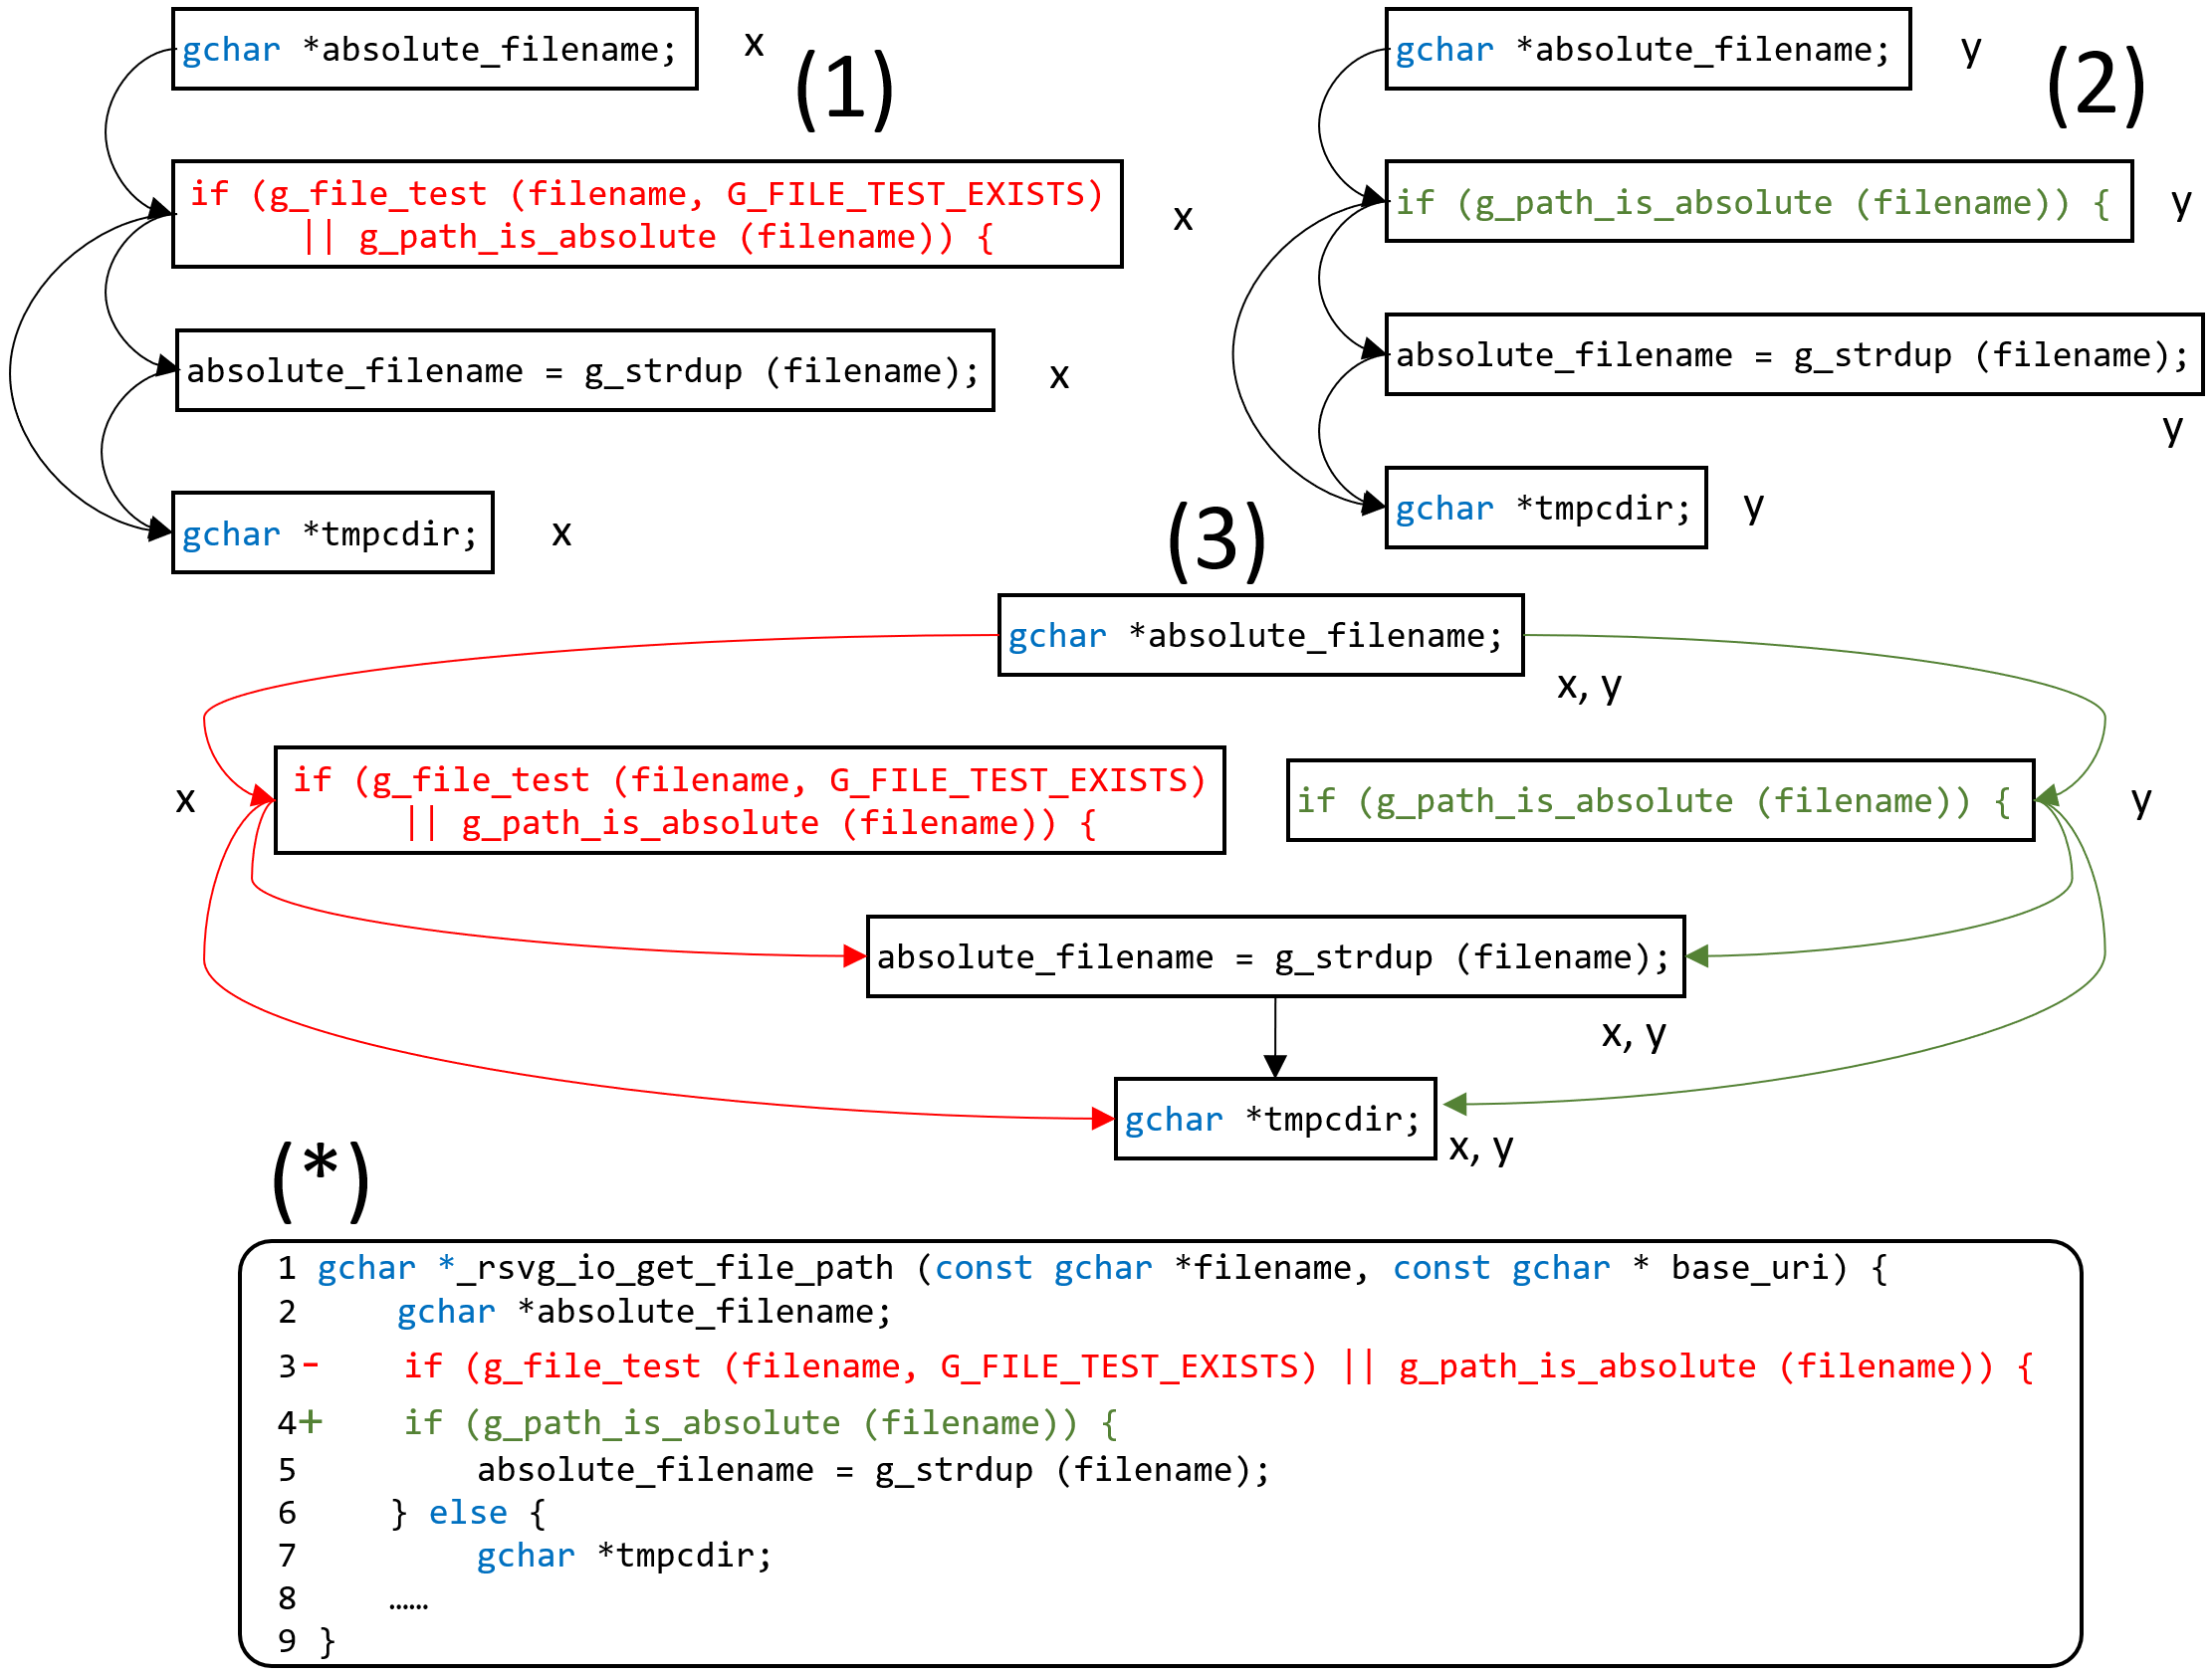
\includegraphics[width=3.4in]{multi-version-pdg.png}
%	\caption{Multi-Version Program Dependence Graph}
%	\label{fig:multi-version-pdg}
%\end{wrapfigure}

For each vulnerability assessment types (VAT), we~have a
SoftMax layer working as an assessment classification model on the
embedding of the entire commit.
%
%the SoftMax layer acts as the classifier, which takes
%the~contextualized embedding for the entire commit built on the
%{\mvpdgxy} and performs classifications.
%
To propagate the impact of the classification for one
assessment type on one another, we leverage multi-task learning among
the classification models. We use the uncertainty weighted multi-task
loss~\cite{kendall2018multi} for each classification task as the final
multi-task learning loss function and use the maximum of the average
F-score from all assessment classification tasks as the
training~target. {\bf Training and Predicting Processes}. The training/predicting processes share the above steps, except
that in training, the classification labels for the
vulnerability-introducing commits w.r.t. a VAT are known. When
predicting, {\tool} takes a vulnerability-introducing commit and code, and provides the assessment classifications for
VATs.        

{\bf Multi-Task Learning for Assessment Classification}
%\label{multi-task:sec}

In the previous sections, we have explained how {\tool} performs the
classification for a vulnerability assessment type (VAT). In this
section, we will explain our multi-task learning mechanism to perform
classifications for all seven VATs with the following prediction
classes for each VAT:

\begin{enumerate}
	\item {\bf Confidentiality}: None; Partial; Complete
	\item {\bf Integrity}: None; Partial; Complete
	\item {\bf Availability}: None; Partial; Complete
	\item {\bf Access Vector}: Local; Network
	\item {\bf Access Complexity}: Low; Medium; High
	\item {\bf Authentication}: None; Single
	\item {\bf Severity}: Low; Medium; High
\end{enumerate}

%\item {\bf Severity}: Low (0.0-3.9); Medium (4.0-6.9); High (7.0-10.0)

%With the SoftMax layer, \tool is able to do the classification for different vulnerability assessment types. In \tool, we follow the existing study DeepCVA \cite{} to do the classification on seven vulnerability assessment types. For each of them, we follows the CVSS's definition on the national vulnerability database \cite{}. These vulnerability assessment types with the classes for each type are listed as follow:

As explained, the vector $v^{com}$
representing the entire commit is passed through a SoftMax layer for
the classification for a specific VAT. Let us call it a classification
task. In CAT, the multi-task learning mechanism uses the uncertainty
weighted multi-task loss~\cite{kendall2018multi} to learn all seven
classification tasks at the same time. Specifically, for each
classification task, \tool uses a cross-entropy loss function to do
the classification as follows:
\begin{equation}\label{new-eq4}
	L = -log(Softmax(y, f(x)))
\end{equation}
Where $f(x)$ is the output of a classification task $f$; y is the
ground truth. To get the joint loss function for seven tasks with
uncertainty weighting, following Kendall {\em et
  al.}'s~\cite{kendall2018multi}, we have
\begin{equation}\label{eq5}
	L_i(W) = -log(Softmax(y_i, f^W(x_i)))
\end{equation}
\begin{equation}\label{eq6}
	L(W, \sigma_1, \sigma_2, ..., \sigma_7) = \sum_{i=1}^7\frac{1}{2\sigma_i^2}L_i(W) + log \sigma^2_i
\end{equation}
Where $W$ is the weight adding to the input, $\sigma_i$ is the
$i^{th}$ noise scalar, and $W$ and $\sigma_i$ are both trainable in
the model. With Formula (\ref{eq6}), {\tool} uses the multi-task
learning to train the seven classification models together with the
features for each task. For training, we set as the objective the
highest average F-score  for all seven
tasks. For prediction, the trained model produces the
classification results for all VATs.
